\documentclass[xcolor=dvipsnames]{beamer}
\usetheme{Rochester}
\usepackage{graphicx}
\usecolortheme[named=OliveGreen]{structure}
\useoutertheme{infolines}
\useinnertheme{rounded}
\setbeamertemplate{blocks}[rounded][shadow=false]
\setbeamertemplate{items}[ball]
\begin{document}
\title[Netsoc Git Tutorial] {Dublin University Internet Society}
\author[A. Anderson \& C. Vize]{Andrew Anderson \inst{1} \and Colm Vize \inst{2}}
\institute[TCD]{\inst{1} School Of Computer Science and Statistics \and \inst{2} Tophat Software}
\subtitle{Git Tutorial}{An introduction to the git VCS}
\date{\today}
\titlepage
\begin{frame}{A tutorial introduction}
	Lets start by creating a repo
	\begin{block}{Create a new repo}
		mkdir myrepo\\
		cd myrepo\\
		git init
	\end{block}
\end{frame}

\begin{frame}{A tutorial introduction}
	
	\begin{block}{Checkout a local repository}
		git clone /path/to/repo
	\end{block}
	\begin{block}{Checkout a remote repository}
		git clone https://github.com/netsoc/Git-Tutorial 
	\end{block}
\end{frame}

\begin{frame}{A tutorial introduction}

	\begin{block}{Workflow}
		Your local repository consists of three "trees" maintained by git. The first one is 
		your \emph{Working Directory} which holds the actual files. the second one is the \emph{Index} which acts as a staging area and finally the \emph{HEAD} which points to the last commit you've made.
	\end{block}
	\begin{center}
		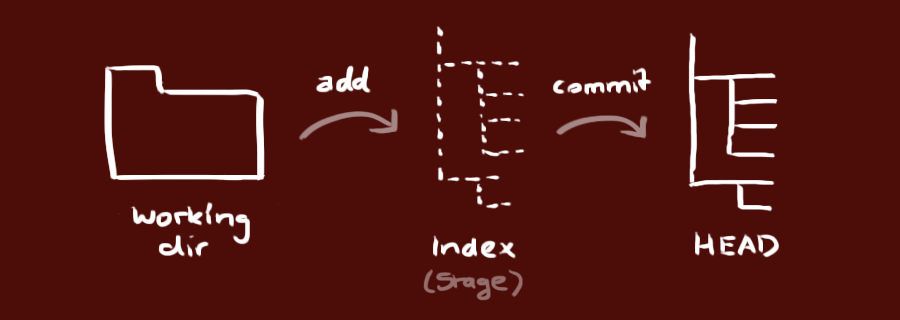
\includegraphics[scale=0.3]{trees.png}
	\end{center}
\end{frame}

\begin{frame}{A tutorial introduction}
	add & commit
You can propose changes (add it to the Index) using
git add <filename>
git add *
This is the first step in the basic git workflow. To actually commit these changes use
git commit -m "Commit message"
Now the file is committed to the HEAD, but not in your remote repository yet.
\date{\today}
\end{frame}
\end{document}
